\documentclass[twoside=false, DIV=14]{scrartcl}

\usepackage{arev} % order matters, putting this above allows FiraSans to override it for body text
\usepackage[sfdefault]{FiraSans}
\usepackage{inconsolata}
%\usepackage[fira]{fontsetup}
\usepackage{scrlayer-scrpage}
\renewcommand{\titlepagestyle}{scrheadings}
\usepackage{graphicx}
\usepackage{blindtext}
\usepackage{wrapfig}
\usepackage{tabularx}
\usepackage{hyperref}
\usepackage{listings}
\usepackage{tikz}
\usepackage{amsmath}
\usepackage[many]{tcolorbox}

\usepackage{xcolor,sectsty}
\definecolor{blackish}{RGB}{56,58,54}
\definecolor{redish}{RGB}{109,41,49}
\definecolor{red}{RGB}{152,41,50}
\definecolor{orangeish}{RGB}{188,71,0}
\definecolor{blueish}{RGB}{25,33,139}
\subsubsectionfont{\color{blackish}}
\subsectionfont{\color{blackish}}
\sectionfont{\color{blackish}}

\lohead{\color{red} COMP3000 Programming Languages}
\rohead{
\includegraphics[width=0.5cm]{../logo.jpg}}

\setkomafont{author}{\sffamily \small}
\setkomafont{date}{\sffamily \small}

\DeclareOldFontCommand{\bf}{\normalfont\bfseries}{\mathbf}
\DeclareOldFontCommand{\tt}{\normalfont\ttfamily}{\texttt}

\lstset{basicstyle=\ttfamily}


\date{}
\newtcolorbox{aside}[1][]{
  title=Aside,
  width=0.3\textwidth,
  fonttitle=\bfseries,
  breakable,
  fonttitle=\bfseries\color{black},
  colframe=blueish!80,
  colback=blueish!2
  #1}

\newtcolorbox{note}[1][]{
  title=Note,
  width=\textwidth,
  fonttitle=\bfseries,
  breakable,
  fonttitle=\bfseries\color{black},
  colframe=orangeish!80,
  colback=orangeish!2
  #1}

\newtcolorbox{hint}[1][]{
    title=Hint,
    width=\textwidth,
    fonttitle=\bfseries,
    breakable,
    fonttitle=\bfseries\color{white},
    colframe=blueish!80,
    colback=blueish!2
    #1}

\newtcolorbox{todo}[1][]{
  title=!! TODO !!,
  width=\textwidth,
  fonttitle=\bfseries,
  breakable,
  fonttitle=\bfseries\color{white},
  colframe=red!80,
  colback=red!2
  #1}
  
\providecommand{\tightlist}{%
  \setlength{\itemsep}{0pt}\setlength{\parskip}{0pt}}

\title{\color{redish} \vspace{-1em}COMP3000 Week 3: The Lox Programming Language}

\begin{document}
{\color{blackish}\maketitle}\vspace{-7em}

\begin{abstract}
This week we turn our focus to the Lox programming language, which will act as our exemplar implemenation over the rest of the semester.  

By the end of this week you should:
\begin{itemize}
    \item Be able to program in Lox
    \item Understand some basic Lox design decisions
\end{itemize}
\end{abstract}

\section*{Topics}
\begin{enumerate}
\item Lox High-Level Features, Typing, and Memory
\item Lox Types, Expressions, and Statements
\item Lox Functions
\item Lox OO Features
\end{enumerate}

\section*{Preparation}
\begin{itemize}
\item Read the text chapters 3
\item Watch lox lectures:
  \begin{itemize}
  \item High level features, types, expressions, and statements.
  \item Functions and OO features
  \item Lox live coding session
  \end{itemize}
\item Complete the RAT individually \emph{and} bring your answers to class.
\item Ensure you have a working lox implementation on your computer.
\item Experiment with lox programs.
\end{itemize}

\newpage
\part*{RAT  \hspace{6em} {\small ANSWER ON ILEARN}}
%\renewcommand{\labelenumii}{\alph{enumii}) $\fbox{$\phantom{x}$}$}
\renewcommand{\labelenumii}{\alph{enumii}) $\square$}
\begin{enumerate}

\item \textbf{output of program}
What will be the output of the following lox program
\begin{lstlisting}
>    var foo = 4;
>    fun simple(){
>        foo = 6;
>    }
>    simple();
>    print foo;
\end{lstlisting}
\begin{enumerate}
    \item \tick 6
    \item 4
    \item compile error due to missing semi-colon
    \item compile error due to wrong keyword
  \end{enumerate}
  
  \item \textbf{Binary Operators}
"binary" operators are so-called because:
\begin{enumerate}
    \item \tick They have two arguments
    \item They work on binary data
    \item They generate binary data
    \item They do arithmetic operations
\end{enumerate}

\item \textbf{Infix Operators}
"infix" operators belong where?
\begin{enumerate}
    \item \tick between the arguments
    \item infix the arguments
    \item within the one argument
    \item after the arguments
\end{enumerate}

\item \textbf{Statement vs Expression}
Match the language feature with its job:
\begin{enumerate}
    \item statement $->$ produce an effect
    \item expression $->$ produce a value
\end{enumerate}

\item \textbf{OO Language Design}
Which of the following approaches to OO language design did the textbook author choose for Lox? :
\begin{enumerate}
    \item \tick  classes
    \item \tick  prototypes
    \item objects
    \item sharing
    \item inheritance
\end{enumerate}
  
\end{enumerate}

\newpage
\part*{Application Exercise}

A fun little language is logo (aka "turtle graphics").  It is a language designed for kids to learn programming.  It has a very simple syntax and a very simple set of commands.  The idea is that you can use it to draw pictures on the screen.  Check out the language this online implementations:
\begin{itemize}
  \item \url{https://www.calormen.com/jslogo/}
\end{itemize}
In this task we will write a lox program which generates logo programs!  To make it interesting, we need to restrict ourselves to using \emph{only} the following logo commands:
\begin{enumerate}
\item \lstinline|clearscreen|: clear the screen
\item \lstinline|fd n|: move the turtle forward n units
\item \lstinline|rt n|: turn the turtle right n degrees
\item \lstinline|pu|: lift the pen up
\item \lstinline|pd|: put the pen down
\end{enumerate}

At the end of class you will share (for either the first task, or your second task) the following:
\begin{enumerate}
  \item The turtle program that was generated
  \item The lox program that generated it.
\end{enumerate}


First, write a lox program which generates a logo program to draw the following picture.  You can use the online logo interpreter to check your generated program.

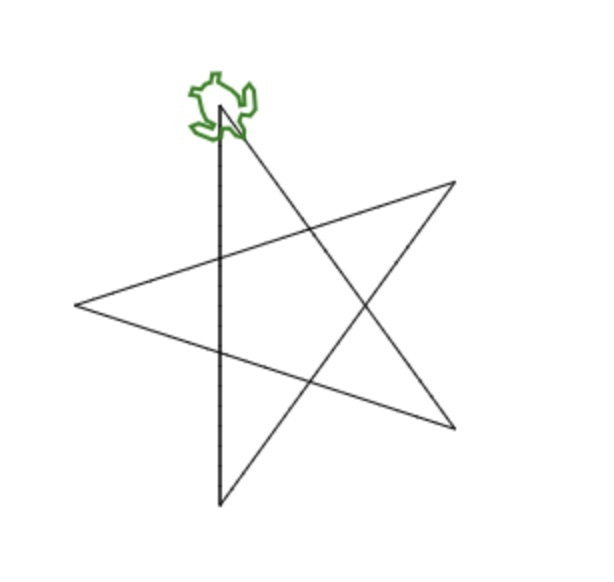
\includegraphics{first.jpg}

Once you have achieved this, try to write a lox program which generates this version.  If using only the commands above, this is a very long program which you don't want to write by hand.  You will \emph{need} to generate this program!

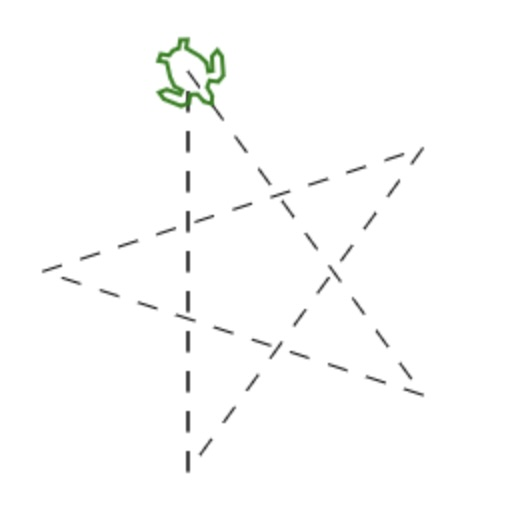
\includegraphics{second.jpg}

Once you have this done, go have some fun with logo and with generating logo programs.  If you have time to come up with a really fun generated program, please share it with the class.

\newpage

\newpage
\part*{Application Exercise Notes and Solutions}

\newpage
\part*{Self Study Exercises}

\section*{Dynamic Types}
The text describes what \emph{dynamic typing} means. Give a definition \emph{in your own words} of that concept.

\subsection*{Solution}
It means the type of a \emph{variable} can change during program execution. It is the opposite of \emph{static} typing where a variable is given a type and it must stay that type. Note that dynamic normally means you don't declare a type, but that is not strictly necessary!

\section*{More General Not More Better}
In the text, the author identifies a language feature which is \emph{simpler} and \emph{more general} than the alternative. Normally we would think of this as an obvious win, but they say it is not. What feature is this and what reason do they give?

\subsection*{Solution}
Choosing classes vs prototyping. They say humans just \emph{seem} to prefer working with classes. This is an important lesson for any language designer—generality and simplicity are \emph{normally} best, but not always. You can only find out with empirical evidence.

\section*{Compile-Time vs Run-Time}
What is \emph{compile time} and what is \emph{run time}? Be precise.

\subsection*{Solution}
"Compile time" is the time between the programmer hitting "compile" and the compiler generating a program. "Run time" is the time between a program starting and the (maybe) program finishing.

\section*{hello world}
  Write a lox program to print "hello world"

\subsection*{Solution}
\begin{lstlisting}
  print "hello world;"  
\end{lstlisting}

\section*{Why Dynamic}
Give a reason dynamic typing might cause more run-time errors than static typing.

\subsection*{Solution}
The text says that "If you try to perform an operation on values of the wrong type — say, dividing a number by a string—then the error is detected and reported at runtime". Other languages could detect this error at compile time.

\section*{Types of Garbage Collection}
Give the name of \emph{one} of the types of garbage collection described in the text.

\subsection*{Solution}
How about two?  \emph{Reference counting} and \emph{tracing}

\section*{Lox programming from the book}
Write some sample Lox programs and run them (you can use the implementations of Lox in my repository). Try to come up with edge case behavior I didn’t specify here. Does it do what you expect? Why or why not?

\subsection*{Solution}
{}

\section*{Square}
Write a Lox program to print the first 50 square numbers.

\subsection*{Solution}
{}

\section*{Prime}
Write a Lox program to print the first 50 prime numbers.

\subsection*{Solution}
{}

\section*{Print to Console}
Write a Lox program which draws a triangle to the console. The first line must be:
\begin{verbatim}
var size = 6
\end{verbatim}
and the \lstinline|size| variable must be used to determine the number of characters on the longest side. For example, \lstinline|size| of 6 prints out:
\begin{verbatim}
******
*****
****
***
**
*
\end{verbatim}

\subsection*{Solution}
{}

\section*{From Book Tiny}
Lox is a pretty tiny language. What features do you think it is missing that would make it annoying to use for real programs? (Aside from the standard library, of course.)

\subsection*{Solution}
{}

\section*{Square Without Loops}
Write a Lox program to print the first 50 square numbers that uses no loops at all.

\subsection*{Solution}
todo

\section*{Prime Without Loops}
Write a Lox program to print the first 50 prime numbers that uses no loops at all.

\subsection*{Solution}
todo

\section*{function}
  Write a lox function \lstinline|foo| which will take in a parameter and return triple that value

\subsection*{Solution}
\begin{lstlisting}
  def foo(val){
      return val*3;
  }
\end{lstlisting}


\section*{repeat}
  Write a lox function \lstinline|repeat| which will take in two parameters.  The first is a string and the second is a number (n).  The function should return the character repeated n times.
\subsection*{Solution}
\begin{lstlisting}
  fun repeat(char, times){
      if (times == 0){
          return "";
      }
      return (char + repeat(char, times-1));
  }
\end{lstlisting}


\section*{Simple Function}
Write a Lox function which takes in a number and returns double that number.

\subsection*{Solution}
\begin{verbatim}
fun double(a) {
    return a + a;
}
\end{verbatim}
I was tricky and used \lstinline|+|. In little languages like Lox, never assume the operator you want is there (though \lstinline|*| is there :).

\section*{Print to Console}
Write a Lox program which draws a triangle to the console without using any loops! The first line must be:
\begin{verbatim}
var size = 6
\end{verbatim}
and the `size` variable must be used to determine the number of characters on the longest side. For example, \lstinline|size| of 6 prints out:
\begin{verbatim}
******
*****
****
***
**
*
\end{verbatim}
Tip: recursion is your friend.

\subsection*{Solution}
\begin{lstlisting}
  var size = 6;

  fun line(len){
      if (len == 0){
          return "";
      } else {
          return ("*" + line(len-1));
      }
  }
  
  fun tri(width){
      if (width == 0){
          return;
      } else {
          print(line(width));
          tri(width-1);
      }
  }
  
  tri(size);  
\end{lstlisting}


\section*{Open Questions}
This informal introduction leaves a lot unspecified. List several open questions you have about the language's syntax and semantics. What do you think the answers should be?

\subsection*{Solution}
{}

\section*{Reason for OO}
Give \emph{your reason} for wanting to have OO in your language. If you hate OO, put yourself in someone else's shoes and think of \emph{their} reason. OO is good enough that you can come up with \emph{something!}

\subsection*{Solution}

\end{document}